\documentclass[a4paper]{book}
\usepackage{lmodern}
\usepackage{amssymb,amsmath}
\usepackage{ifxetex,ifluatex}
\usepackage{fixltx2e} % provides \textsubscript
\ifnum 0\ifxetex 1\fi\ifluatex 1\fi=0 % if pdftex
  \usepackage[T1]{fontenc}
  \usepackage[utf8]{inputenc}
\else % if luatex or xelatex
  \ifxetex
    \usepackage{mathspec}
  \else
    \usepackage{fontspec}
  \fi
  \defaultfontfeatures{Ligatures=TeX,Scale=MatchLowercase}
\fi
% use upquote if available, for straight quotes in verbatim environments
\IfFileExists{upquote.sty}{\usepackage{upquote}}{}
% use microtype if available
\IfFileExists{microtype.sty}{%
\usepackage{microtype}
\UseMicrotypeSet[protrusion]{basicmath} % disable protrusion for tt fonts
}{}
\usepackage[margin=1in]{geometry}
\usepackage{hyperref}
\hypersetup{unicode=true,
            pdftitle={Introducción al diseño y análisis de experimentos usando R},
            pdfauthor={Agustín Alesso},
            pdfborder={0 0 0},
            breaklinks=true}
\urlstyle{same}  % don't use monospace font for urls
\usepackage{natbib}
\bibliographystyle{apalike}
\usepackage{color}
\usepackage{fancyvrb}
\newcommand{\VerbBar}{|}
\newcommand{\VERB}{\Verb[commandchars=\\\{\}]}
\DefineVerbatimEnvironment{Highlighting}{Verbatim}{commandchars=\\\{\}}
% Add ',fontsize=\small' for more characters per line
\usepackage{framed}
\definecolor{shadecolor}{RGB}{248,248,248}
\newenvironment{Shaded}{\begin{snugshade}}{\end{snugshade}}
\newcommand{\AlertTok}[1]{\textcolor[rgb]{0.94,0.16,0.16}{#1}}
\newcommand{\AnnotationTok}[1]{\textcolor[rgb]{0.56,0.35,0.01}{\textbf{\textit{#1}}}}
\newcommand{\AttributeTok}[1]{\textcolor[rgb]{0.77,0.63,0.00}{#1}}
\newcommand{\BaseNTok}[1]{\textcolor[rgb]{0.00,0.00,0.81}{#1}}
\newcommand{\BuiltInTok}[1]{#1}
\newcommand{\CharTok}[1]{\textcolor[rgb]{0.31,0.60,0.02}{#1}}
\newcommand{\CommentTok}[1]{\textcolor[rgb]{0.56,0.35,0.01}{\textit{#1}}}
\newcommand{\CommentVarTok}[1]{\textcolor[rgb]{0.56,0.35,0.01}{\textbf{\textit{#1}}}}
\newcommand{\ConstantTok}[1]{\textcolor[rgb]{0.00,0.00,0.00}{#1}}
\newcommand{\ControlFlowTok}[1]{\textcolor[rgb]{0.13,0.29,0.53}{\textbf{#1}}}
\newcommand{\DataTypeTok}[1]{\textcolor[rgb]{0.13,0.29,0.53}{#1}}
\newcommand{\DecValTok}[1]{\textcolor[rgb]{0.00,0.00,0.81}{#1}}
\newcommand{\DocumentationTok}[1]{\textcolor[rgb]{0.56,0.35,0.01}{\textbf{\textit{#1}}}}
\newcommand{\ErrorTok}[1]{\textcolor[rgb]{0.64,0.00,0.00}{\textbf{#1}}}
\newcommand{\ExtensionTok}[1]{#1}
\newcommand{\FloatTok}[1]{\textcolor[rgb]{0.00,0.00,0.81}{#1}}
\newcommand{\FunctionTok}[1]{\textcolor[rgb]{0.00,0.00,0.00}{#1}}
\newcommand{\ImportTok}[1]{#1}
\newcommand{\InformationTok}[1]{\textcolor[rgb]{0.56,0.35,0.01}{\textbf{\textit{#1}}}}
\newcommand{\KeywordTok}[1]{\textcolor[rgb]{0.13,0.29,0.53}{\textbf{#1}}}
\newcommand{\NormalTok}[1]{#1}
\newcommand{\OperatorTok}[1]{\textcolor[rgb]{0.81,0.36,0.00}{\textbf{#1}}}
\newcommand{\OtherTok}[1]{\textcolor[rgb]{0.56,0.35,0.01}{#1}}
\newcommand{\PreprocessorTok}[1]{\textcolor[rgb]{0.56,0.35,0.01}{\textit{#1}}}
\newcommand{\RegionMarkerTok}[1]{#1}
\newcommand{\SpecialCharTok}[1]{\textcolor[rgb]{0.00,0.00,0.00}{#1}}
\newcommand{\SpecialStringTok}[1]{\textcolor[rgb]{0.31,0.60,0.02}{#1}}
\newcommand{\StringTok}[1]{\textcolor[rgb]{0.31,0.60,0.02}{#1}}
\newcommand{\VariableTok}[1]{\textcolor[rgb]{0.00,0.00,0.00}{#1}}
\newcommand{\VerbatimStringTok}[1]{\textcolor[rgb]{0.31,0.60,0.02}{#1}}
\newcommand{\WarningTok}[1]{\textcolor[rgb]{0.56,0.35,0.01}{\textbf{\textit{#1}}}}
\usepackage{longtable,booktabs}
\usepackage{graphicx,grffile}
\makeatletter
\def\maxwidth{\ifdim\Gin@nat@width>\linewidth\linewidth\else\Gin@nat@width\fi}
\def\maxheight{\ifdim\Gin@nat@height>\textheight\textheight\else\Gin@nat@height\fi}
\makeatother
% Scale images if necessary, so that they will not overflow the page
% margins by default, and it is still possible to overwrite the defaults
% using explicit options in \includegraphics[width, height, ...]{}
\setkeys{Gin}{width=\maxwidth,height=\maxheight,keepaspectratio}
\IfFileExists{parskip.sty}{%
\usepackage{parskip}
}{% else
\setlength{\parindent}{0pt}
\setlength{\parskip}{6pt plus 2pt minus 1pt}
}
\setlength{\emergencystretch}{3em}  % prevent overfull lines
\providecommand{\tightlist}{%
  \setlength{\itemsep}{0pt}\setlength{\parskip}{0pt}}
\setcounter{secnumdepth}{5}
% Redefines (sub)paragraphs to behave more like sections
\ifx\paragraph\undefined\else
\let\oldparagraph\paragraph
\renewcommand{\paragraph}[1]{\oldparagraph{#1}\mbox{}}
\fi
\ifx\subparagraph\undefined\else
\let\oldsubparagraph\subparagraph
\renewcommand{\subparagraph}[1]{\oldsubparagraph{#1}\mbox{}}
\fi

%%% Use protect on footnotes to avoid problems with footnotes in titles
\let\rmarkdownfootnote\footnote%
\def\footnote{\protect\rmarkdownfootnote}

%%% Change title format to be more compact
\usepackage{titling}

% Create subtitle command for use in maketitle
\newcommand{\subtitle}[1]{
  \posttitle{
    \begin{center}\large#1\end{center}
    }
}

\setlength{\droptitle}{-2em}

  \title{Introducción al diseño y análisis de experimentos usando R}
    \pretitle{\vspace{\droptitle}\centering\huge}
  \posttitle{\par}
    \author{Agustín Alesso}
    \preauthor{\centering\large\emph}
  \postauthor{\par}
    \date{}
    \predate{}\postdate{}
  
\usepackage[spanish]{babel}
\usepackage[utf8]{inputenc}
\usepackage{booktabs}
\usepackage{amsthm}
\makeatletter
\def\thm@space@setup{%
  \thm@preskip=8pt plus 2pt minus 4pt
  \thm@postskip=\thm@preskip
}
\makeatother

\begin{document}
\maketitle

{
\setcounter{tocdepth}{1}
\tableofcontents
}
\hypertarget{introduccion}{%
\chapter*{Introducción}\label{introduccion}}
\addcontentsline{toc}{chapter}{Introducción}

Este pequeño libro tiene como objetivo servir como material de apoyo al
curso de Diseños de Experimentos de la Maestría de Cultivos Intensivos
de la FCA-UNL. En el se desarrollará

Introducción a R/Rstudio Repaso de estadística básica Principios de
diseño Diseǹos más empleados

Al final del libro se espera que Ud.

\begin{itemize}
\tightlist
\item
  Reconozca la importancia del enfoque estadístico para el diseño de
  experimentos
\item
  Tenga un sólido entendimiento de los principales métodos utilizados
  para el análisis de datos provenientes de experimentos diseñados.
\item
  Desarrolle destrezas mínimas para utilizar el paquete estadístico R y
  el entorno de trabajo RStudio.
\item
  Sepa interpretar los resultados de los análisis estadísticos en
  contexto de las ciencias biológicas y agrícolas.
\end{itemize}

\hypertarget{empezando-con-r-y-rstudio}{%
\chapter{Empezando con R y RStudio}\label{empezando-con-r-y-rstudio}}

R es un lenguaje y entorno para el procesamiento, visualización y
análisis estadístico de datos. Ha sido creado en 1993 por R. Gentleman y
R. Ihaka, ambos científicos del Departamento de Estadística de la
Universidad de Auckland (Nueva Zelanda). Actualmente su desarrollo y
mantenimiento está a cargo del \emph{R Core Team}. El sitio oficial del
proyecto es \url{www.r-project.org}

\begin{figure}[h]

{\centering 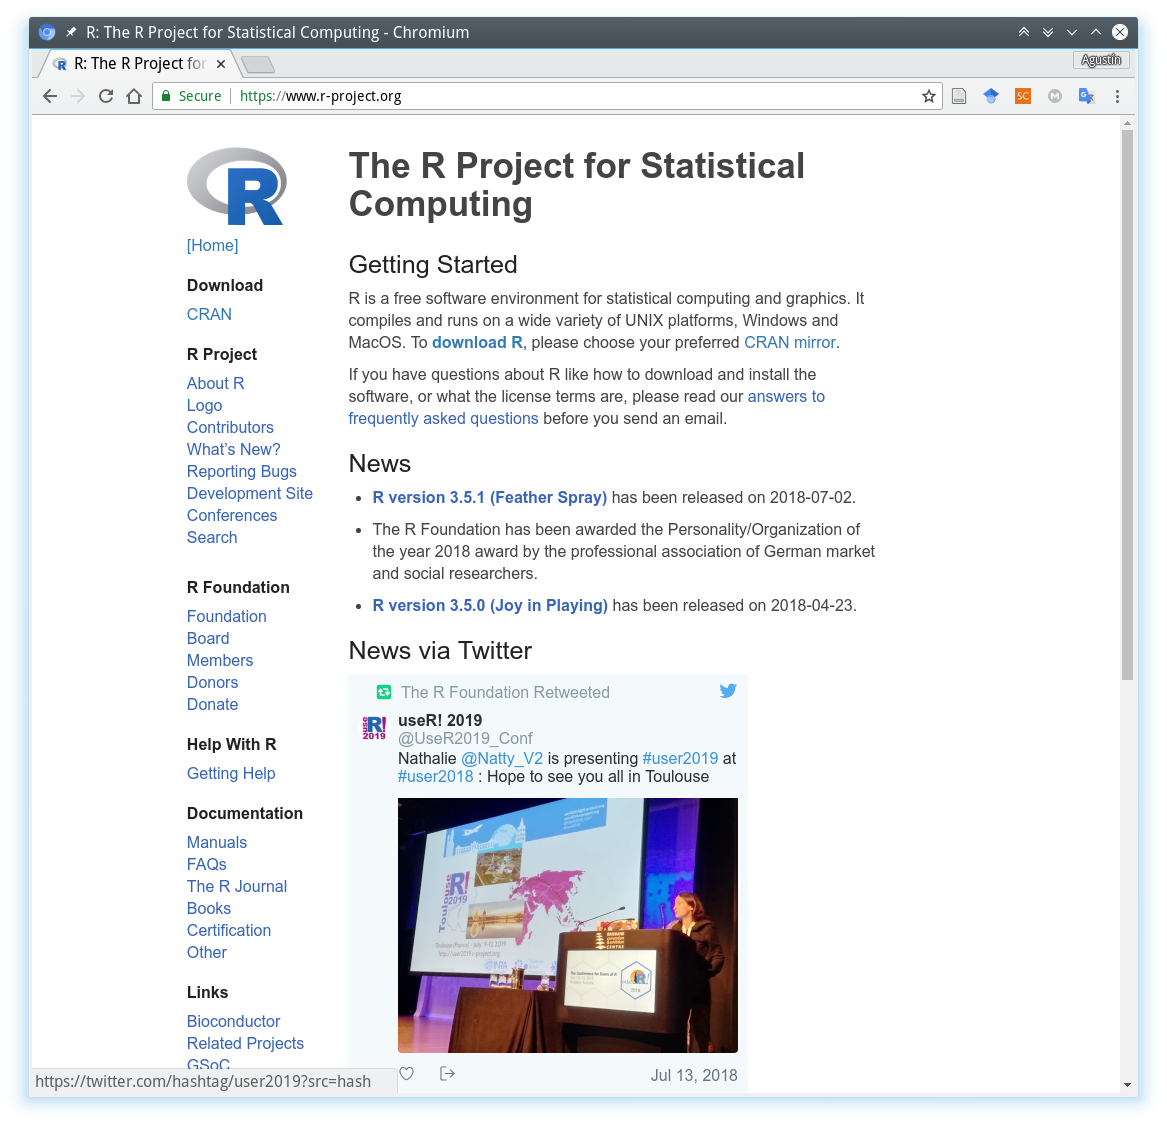
\includegraphics[width=0.75\linewidth,]{images/rproject} 

}

\caption{Página oficial de R Project}\label{fig:unnamed-chunk-2}
\end{figure}

Hoy en día, R es la \emph{lingua franca} del procesamiento y análisis
estadístico de datos, tanto en el ámbito académico como comercial dado
que es gratiuto, multiplataforma, de código abierto (\emph{open source},
liberado con licencia GNU/GPL). Esto lo convierte en un software muy
potente y que expresa el estado del arte de los métodos estadísticos ya
que la comunidad de usuarios contribuya constantemente con
funcionalidades e implementaciones de nuevos métodos y técnicas
estadísticas.

Al igual que su antecesor S, la flexibilidad y potencia de R se basa en
su interfaz de comandos (CLI, del inglés \emph{command line interface} )
que permite la ejecución de comandos de manera interactiva (en consola)
o automática mediante scritps.

\begin{figure}[h]

{\centering 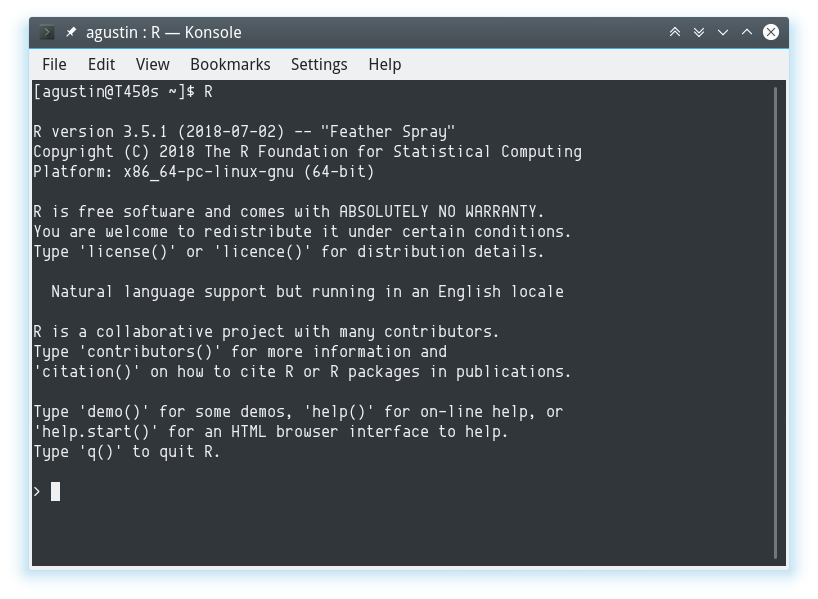
\includegraphics[width=0.75\linewidth,]{images/consola_linux} 

}

\caption{Consola o terminal de Windows, Mac OS X y Linux corriendo la última versión estable de R}\label{fig:unnamed-chunk-31}
\end{figure}
\begin{figure}[h]

{\centering 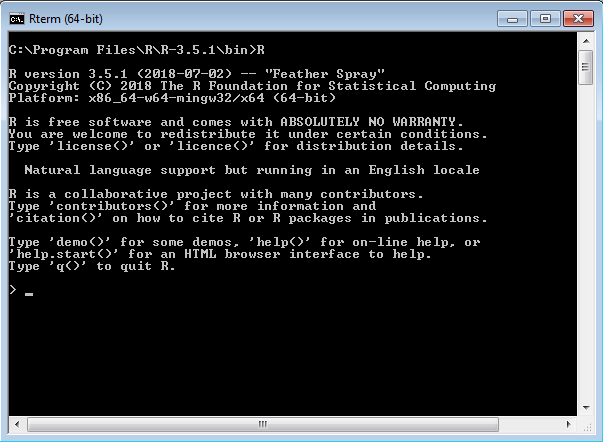
\includegraphics[width=0.75\linewidth,]{images/consola_windows} 

}

\caption{Consola o terminal de Windows, Mac OS X y Linux corriendo la última versión estable de R}\label{fig:unnamed-chunk-32}
\end{figure}

Existen algunos desarrollos de interfases gráficas (GUIs, del inglés
\emph{graphical user interface}), e.g.~RCommander, Deducer, que ofrecen
la posibilidad de, mediante menues y botones, ejecutar análisis
relativamente simples minimizando la necesidad de escribir código.

\begin{figure}[h]

{\centering 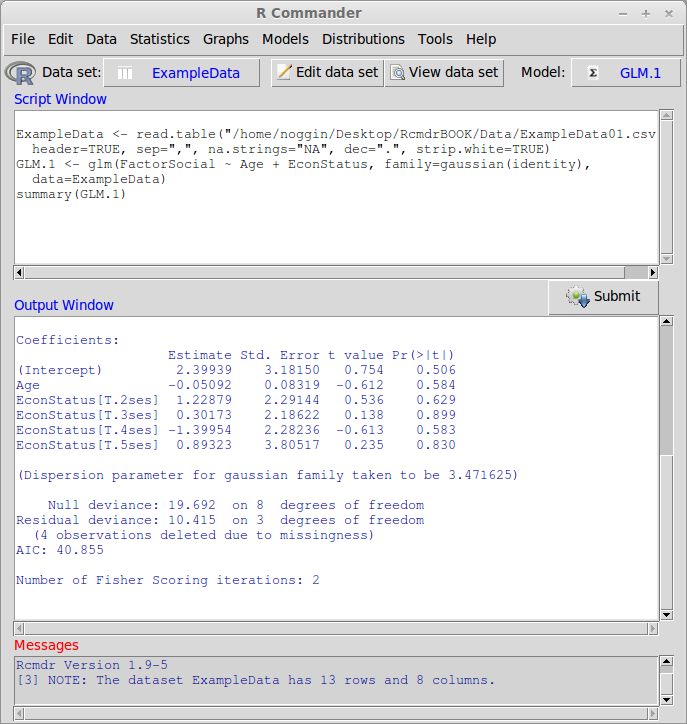
\includegraphics[width=0.75\linewidth,]{images/RcmdrBASE} 

}

\caption{Interfase de R Commander}\label{fig:unnamed-chunk-4}
\end{figure}

Por su parte, los entornos de desarrollo integrados (IDE por sus siglas
en inglés \emph{integrated development environments}) ofrecen un enfoque
intermedio con menúes o funciones asistentes que facilitan algunas
tareas generales (abrir archivos, carga de datos, exportar gráficos y
resultados) pero dejando la codificación del análisis estadístico en
manos del usuario mediante la ejecución de scripts. Entre estas
alternativas se destaca RStudio ( \url{www.rstudio.com} ) el cual
también es de código abierto (licencia GNU/GPL), multiplataforma y
ofrece una versión gratuita.

\begin{figure}[h]

{\centering \includegraphics[width=0.75\linewidth,]{images/RStudio} 

}

\caption{Interfase de RStudio}\label{fig:unnamed-chunk-5}
\end{figure}

\hypertarget{como-instalar-r-y-rstudio}{%
\section{¿Cómo instalar R y RStudio?}\label{como-instalar-r-y-rstudio}}

RStudio requiere que el sistema tenga al menos una versión de R
instalada. Ambos softwares son multiplataforma y pueden ser ejecutados
en sistemas operativos Windows, OS X y Linux. A continuación se describe
el procedimiento para instalar R y RStudio bajo Windows.

\hypertarget{instalacion-de-r}{%
\subsection{Instalación de R}\label{instalacion-de-r}}

\begin{enumerate}
\def\labelenumi{\arabic{enumi})}
\tightlist
\item
  Descargar el archivo instalador correspondiente a la última versión
  estable de R desde el CRAN\footnote{CRAN se compone de un conjunto de
    servidores espejo distribuidos alrededor del mundo que tienen copias
    de R y sus paquetes. No es necesario escojer el espejo más cercano
    ya que el espejo nube (\url{https://cloud.r-project.org})
    automáticamente determina de que servidor conviene realizar la
    descarga.} (del inglés, \emph{Comprenhensive R Archive Network})
  visitando el siguiente
  \href{https://cloud.r-project.org/bin/windows/base/release.htm}{link}
  \footnote{Al momento de escribir estas instrucciones la última versión
    estable de R era la 3.5.1 ``Feather Spray'', por lo tanto el link
    apuntará al archivo \texttt{R-3.5.1-win.exe}.}.
\end{enumerate}

\begin{figure}[h]

{\centering 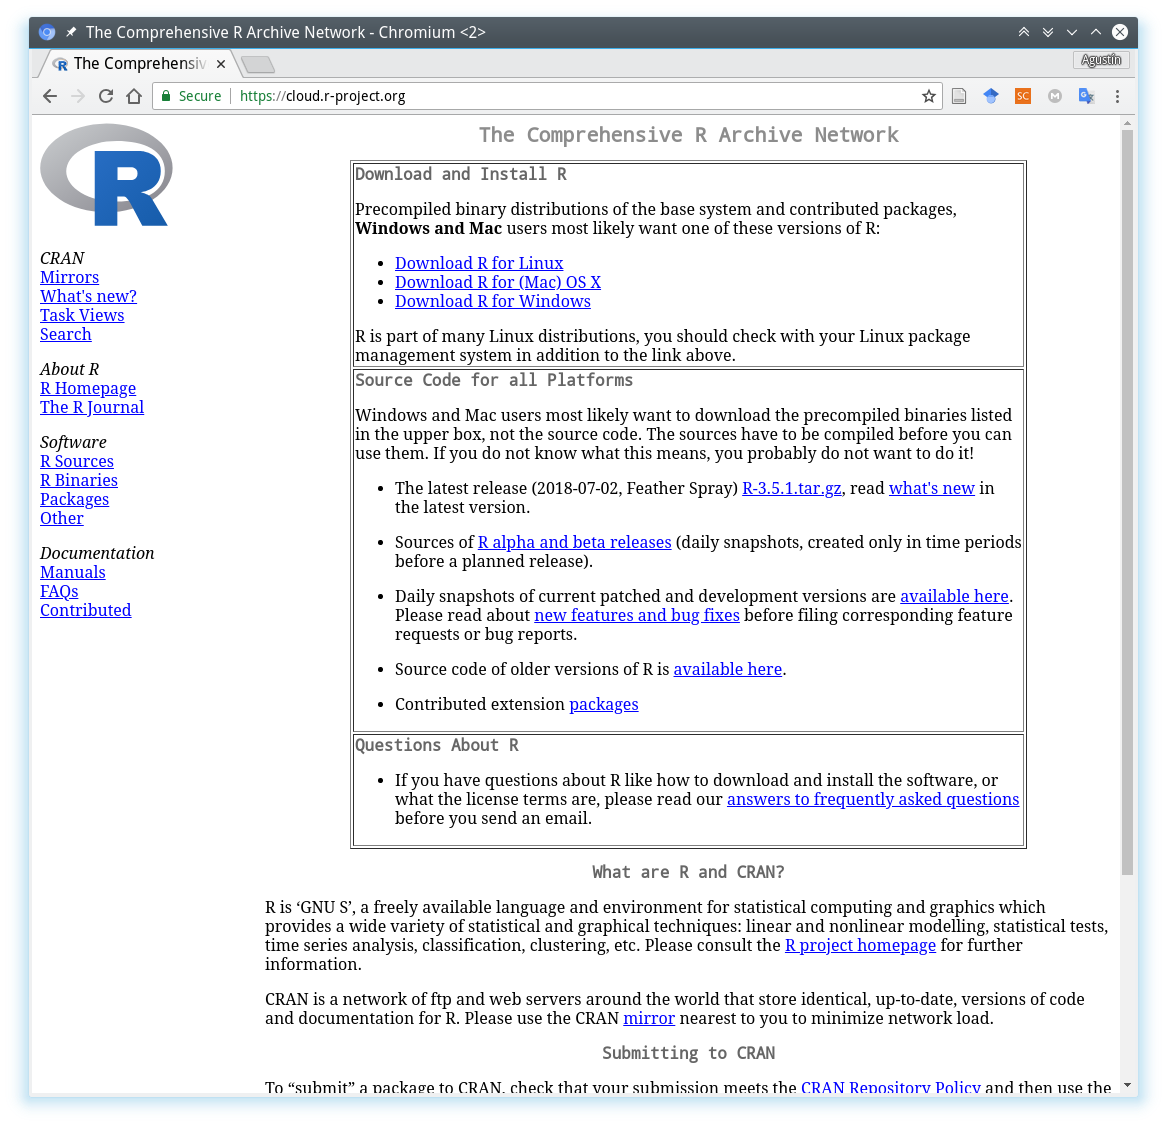
\includegraphics[width=0.75\linewidth,]{images/choose_OS} 

}

\caption{Página de descaga de R}\label{fig:unnamed-chunk-6}
\end{figure}

\begin{enumerate}
\def\labelenumi{\arabic{enumi})}
\setcounter{enumi}{1}
\item
  Una vez finalizada la descarga ejecutar el archivo \texttt{.exe} y
  seguir el asistente de instalación con todas las opciones por defecto.

  Si la instalación ha sido exitosa el el menú \emph{Inicio
  \textgreater{} Todos los Programas \textgreater{} R} se encontrarán
  dos accesos directos \texttt{R\ i386\ 3.5.1} y \texttt{R\ x64\ 3.5.1}
  los cuales permiten correre la interfase de usuario mínima que viene
  con la versión de R para Windows.
\end{enumerate}

\begin{figure}[h]

{\centering 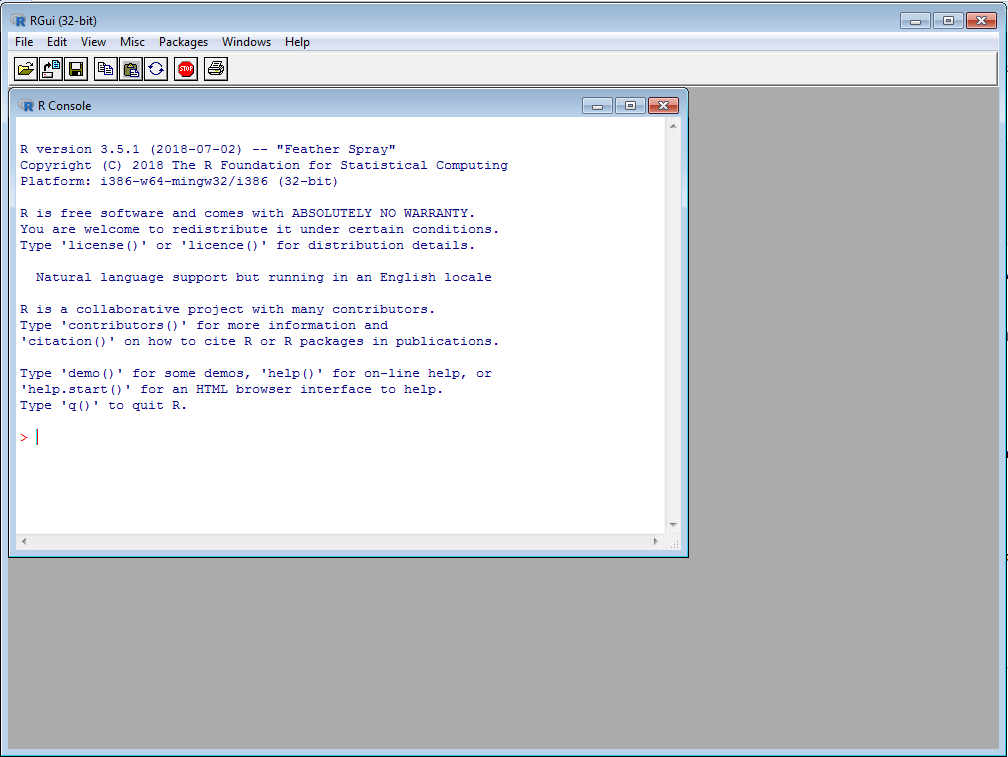
\includegraphics[width=0.75\linewidth,]{images/rgui} 

}

\caption{R GUI para Windows}\label{fig:unnamed-chunk-7}
\end{figure}

\hypertarget{instalacion-de-rstudio}{%
\subsection{Instalación de RStudio}\label{instalacion-de-rstudio}}

\begin{enumerate}
\def\labelenumi{\arabic{enumi})}
\tightlist
\item
  Ir al sitio web de descarga de RStudio:
  \url{https://www.rstudio.com/products/rstudio/download/}
\end{enumerate}

\begin{figure}[h]

{\centering 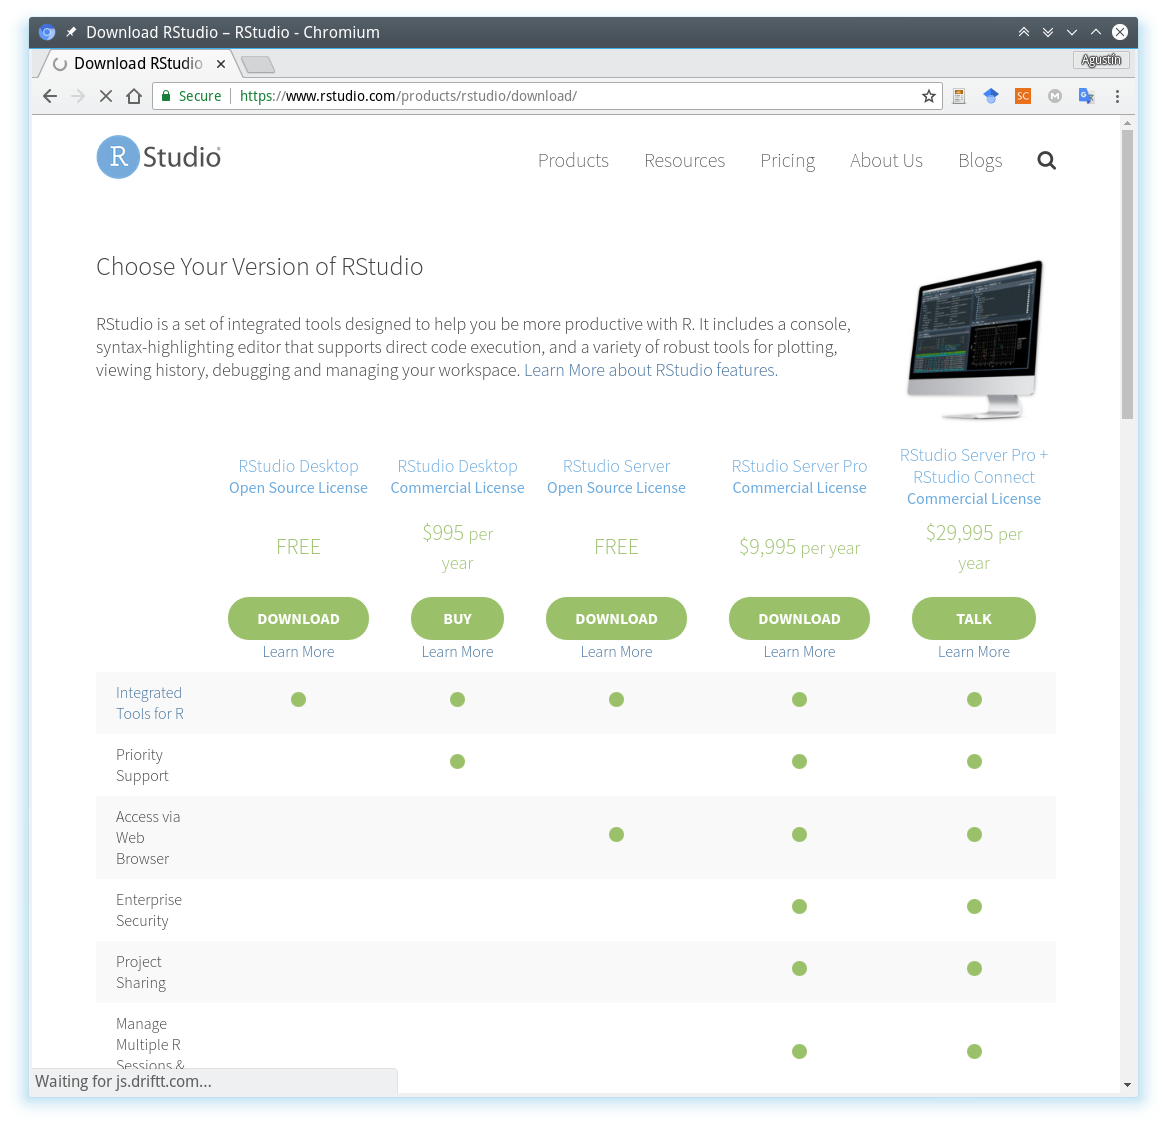
\includegraphics[width=0.75\linewidth,]{images/rstudio_download} 

}

\caption{Página principal de RStudio}\label{fig:unnamed-chunk-8}
\end{figure}

\begin{enumerate}
\def\labelenumi{\arabic{enumi})}
\setcounter{enumi}{1}
\tightlist
\item
  Descargar el archivo de instalación correspondiente a nuestra
  plataforma o sistema operativo. Por ejemplo: para Windows iniciará la
  descarga del archivo \texttt{RStudio-1.1.453.exe}
\end{enumerate}

\begin{figure}[h]

{\centering 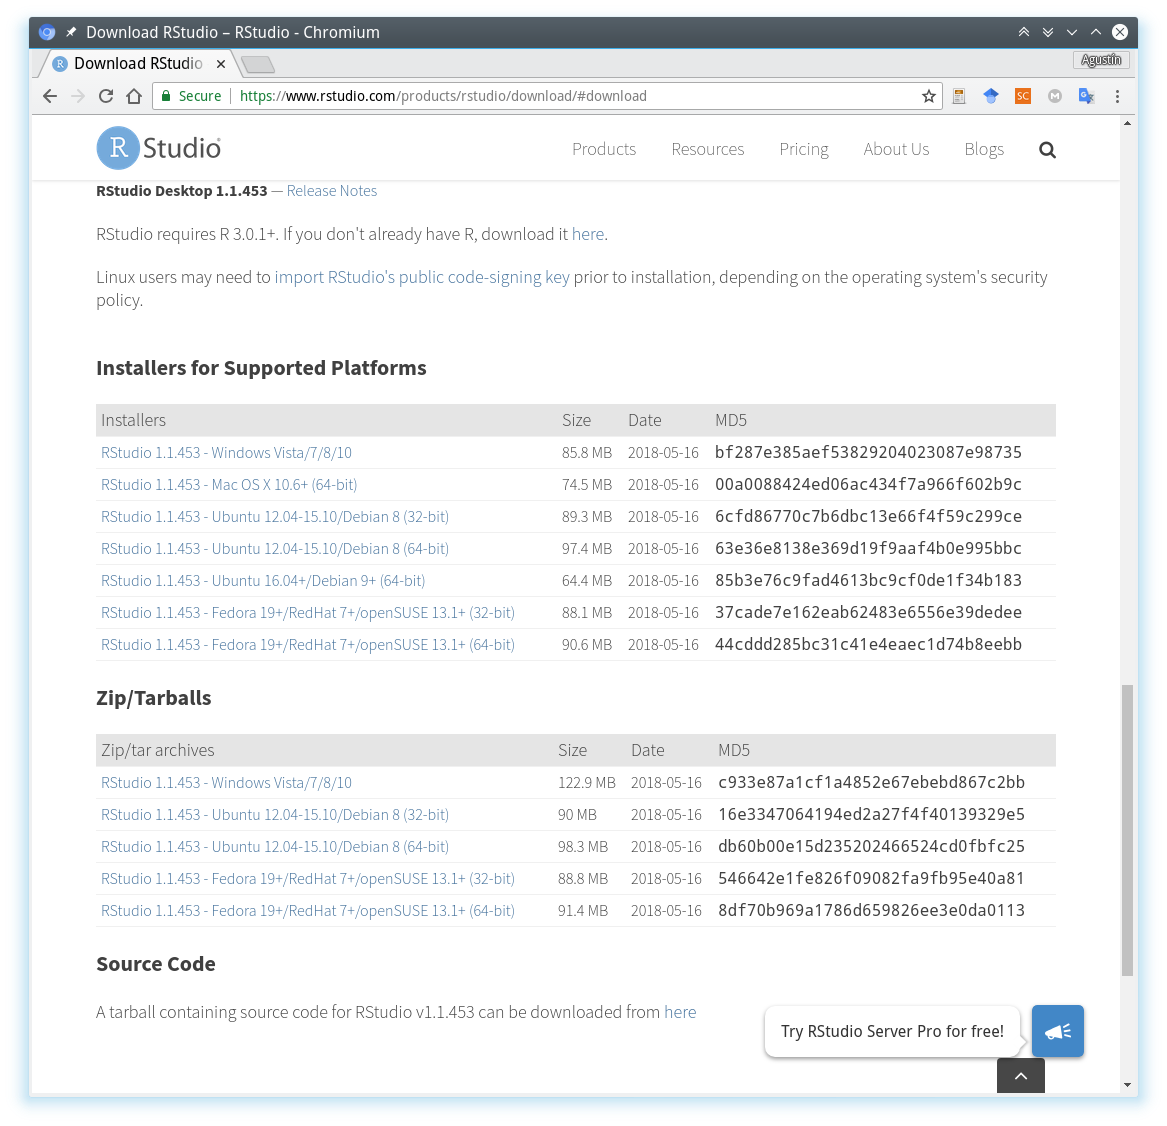
\includegraphics[width=0.75\linewidth,]{images/rstudio_download_OS} 

}

\caption{Página principal de RStudio}\label{fig:unnamed-chunk-9}
\end{figure}

\begin{enumerate}
\def\labelenumi{\arabic{enumi})}
\setcounter{enumi}{2}
\tightlist
\item
  Una vez finalizada la descarga ejecutar el archivo \texttt{.exe}
  \footnote{Al momento de escribir estas instrucciones la última versión
    estable de R Studio era la 1.1.453 por lo tanto el link apuntará al
    archivo \texttt{RStudio-1.1.453.exe}.} \texttt{RStudio-1.1.453.exe}
  y seguir el asistente de instalación con todas las opciones por
  defecto.
\end{enumerate}

Si la instalación ha sido exitosa el el menú \emph{Inicio \textgreater{}
Todos los Programas \textgreater{} RStudio} se encontrará el acceso
directo a RStudio el cual, mediante el menu contextual (botón derecho
del ratón) puede enviarse al Escritorio como acceso directo o bien
anclar al menu de Inicio o barra de acceso rápido.

Ahora sí, ya tenemos listo R y RStudio para empezar a trabajar!!

\hypertarget{primera-sesion-en-rstudio}{%
\section{Primera sesión en RStudio}\label{primera-sesion-en-rstudio}}

El entorno de trabajo de RStudio se divide en cuatro paneles: (1) el
editor, (2) la consola, (3) entorno, historia de comandos y conexiones y
(4) administrador de archivos, gráficos, ayuda y paquetes.

\begin{figure}[h]

{\centering 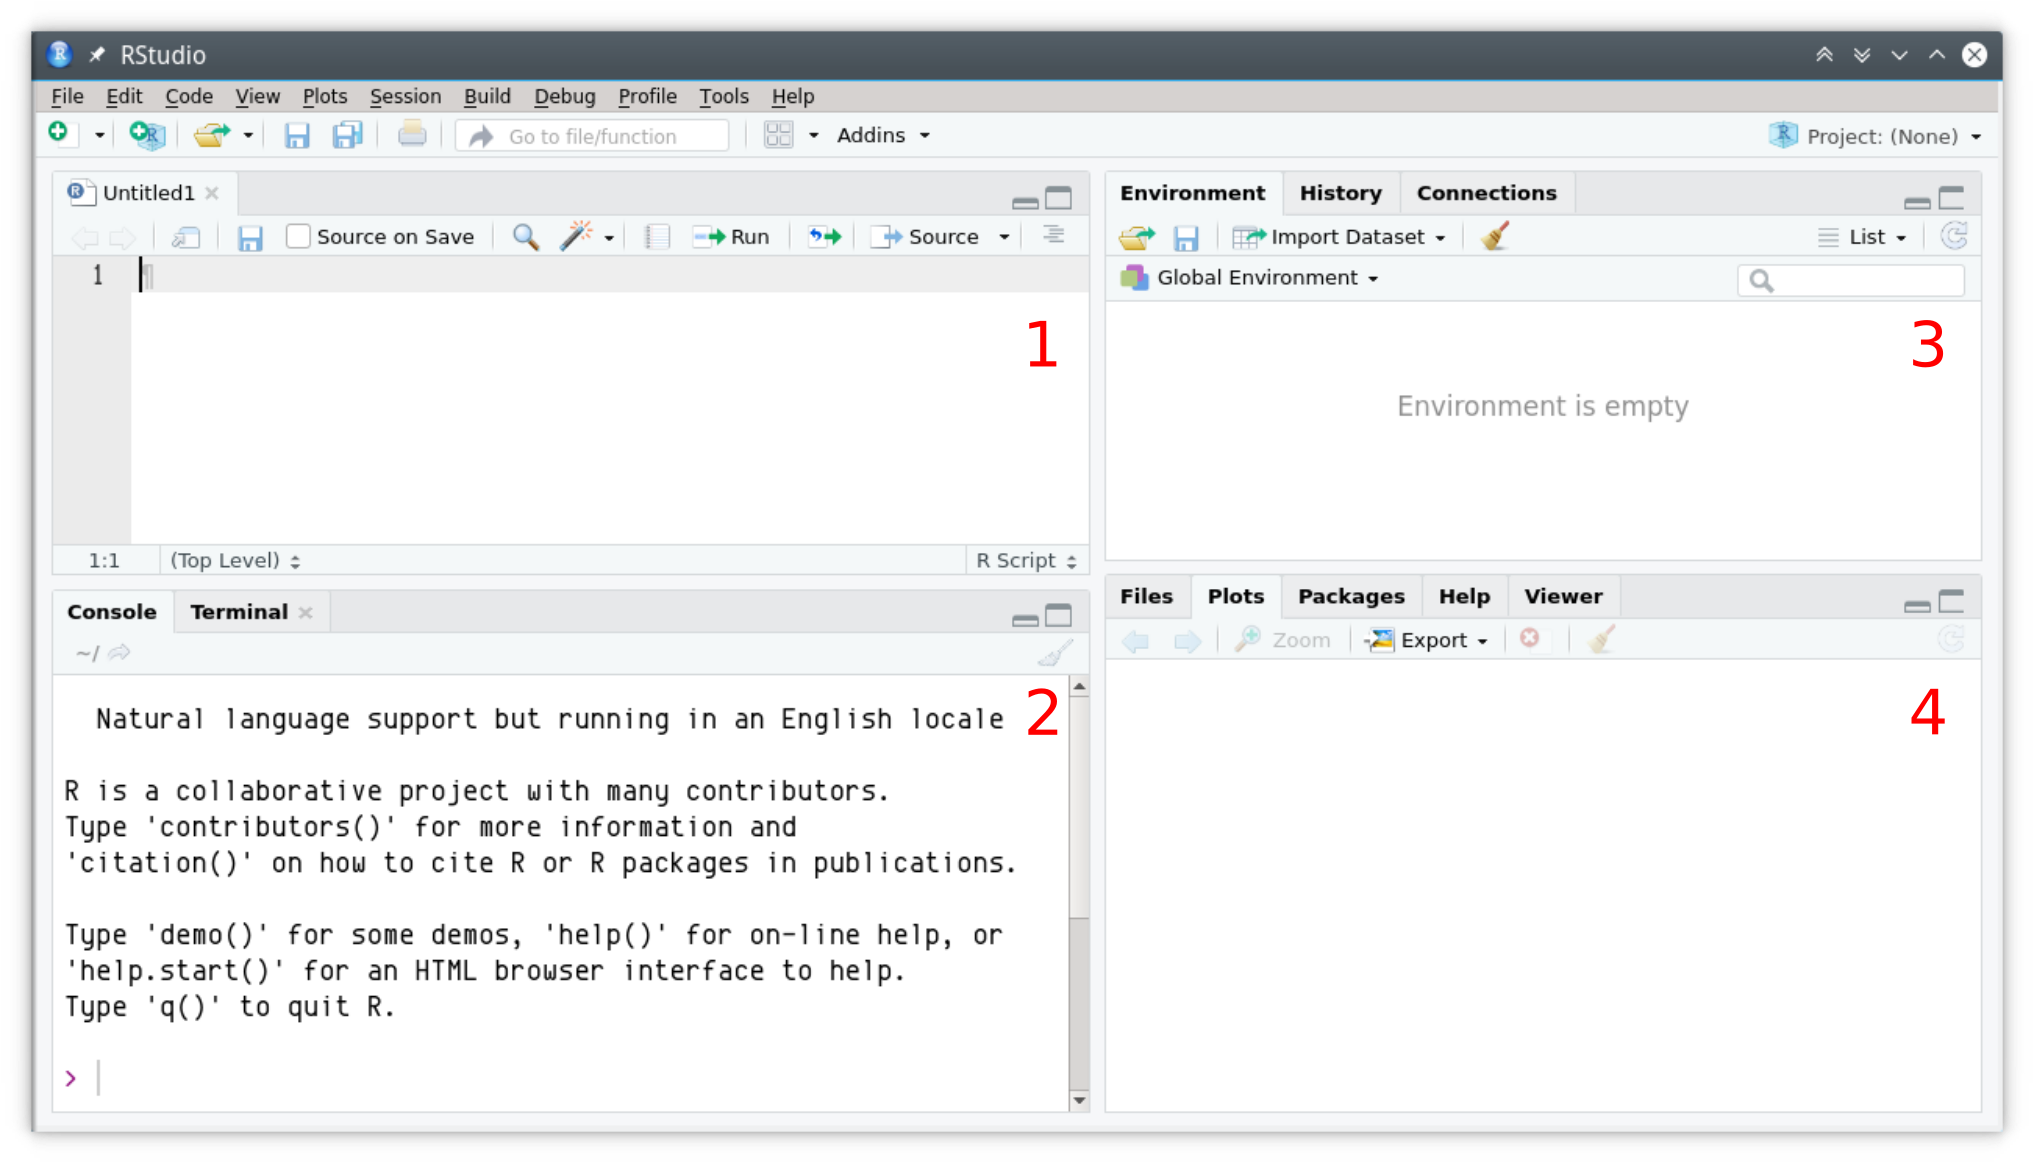
\includegraphics[width=0.75\linewidth,]{images/RStudio_paneles} 

}

\caption{Interfase principal de RStudio}\label{fig:unnamed-chunk-10}
\end{figure}

\begin{enumerate}
\def\labelenumi{\arabic{enumi}.}
\item
  \textbf{Editor de scripts}. Por defecto este panel no aparece a menos
  que se cree un nuevo script o se abra uno previamente guardado. Es
  básicamente un editor de texto plano como el block de notas, aunque
  tiene algunas funcionalidades importantes:

  \begin{itemize}
  \tightlist
  \item
    Resaltado sintaxis: mediante colores resalta las funciones,
    variables, comandos o palabras claves del lenguaje \textbf{R}
  \item
    Sangrado automático: agrega espacios en blanco para mantener la
    sangría de los bloques de código.
  \item
    Completado automático: muestra sugerencias para completar el comando
    o argumentos usando la tecla \texttt{TAB}.
  \end{itemize}
\item
  \textbf{Consola}. Es donde reside \textbf{R} propiamente dicho. Allí
  se ejecutan los comandos y se obtienen las salidas de \textbf{R}. El
  símbolo es \texttt{\textgreater{}} indica que \textbf{R} está
  disponible para recibir un comando que ouede ser tipeado directamente,
  o bien enviado desde el editor de scripts usando la combinación
  \texttt{CTRL\ +\ ENTER} o \texttt{CTRL\ +\ R}.
\item
  \textbf{Environmnet/History}. En la primera pestaña se visualizan los
  objetos (variables, funciones o datos cargados) en el entorno de
  \textbf{R}. En la segunda se puede ver el historial de comandos
  ingresados o enviados a la consola
\item
  \textbf{Files/Plots/Packages/Help/Viewer}. Allí se puede manejar los
  archivos del directorio de trabajo, visualizar los gráficos generados
  en \textbf{R} con posibilidad de exportarlos en varios formatos,
  administrar los paquetes o complementos, buscar o explorar el manual
  de ayuda.
\end{enumerate}

\hypertarget{crear-un-proyecto}{%
\subsection{Crear un Proyecto}\label{crear-un-proyecto}}

Antes de comenzar es conveniente crear un proyecto dentro de
\textbf{RStudio}. Esto permitirá organizar los archivos de datos, las
salidas, los scripts, etc., dentro de un directorio de trabajo
(\emph{working directory}) y volver a ellos de manera más rápida y
eficiente.

\begin{enumerate}
\def\labelenumi{\arabic{enumi}.}
\item
  Ir a \texttt{File\ \textgreater{}\ New\ project...} o bien el ícono
  \texttt{New\ project}.
\item
  Luego seleccionar \texttt{New\ directory} y \texttt{Empty\ project}
\item
  Una vez en el cuadro de diálogo \texttt{Create\ new\ project}
\end{enumerate}

En \texttt{Directory\ name} ingresar el nombre del proyecto (e.g.
\texttt{Diseño2016}) que será a su vez el nombre de la carpeta que
\textbf{RStudio} va a crear.

Luego en \texttt{Create\ project\ as\ a\ subdirectory\ of} vamos indicar
\textbf{donde} queremos que \textbf{Rstudio} cree la carpeta.

\begin{enumerate}
\def\labelenumi{\arabic{enumi}.}
\setcounter{enumi}{3}
\tightlist
\item
  Si todo sale bien, se crea la carpeta con el nombre que indicamos y
  dentro de ésta un archivo con extensión \texttt{.Rproj}
\end{enumerate}

\hypertarget{modo-interactivo-la-consola}{%
\subsection{Modo interactivo: la
consola}\label{modo-interactivo-la-consola}}

La línea de comando o \textbf{consola} es el modo interactivo mediante
el cual podemos ejecutar comandos directamente en el intérprete de
\textbf{R}. El símbolo \texttt{\textgreater{}} indica que \textbf{R}
está disponible esperando una orden. Si la orden no está completa el
símbolo se transoforma en \texttt{+}. Por ejemplo: \texttt{2\ +\ 2}

\begin{Shaded}
\begin{Highlighting}[]
\DecValTok{2} \OperatorTok{+}\StringTok{ }\DecValTok{2}
\end{Highlighting}
\end{Shaded}

\begin{verbatim}
## [1] 4
\end{verbatim}

Otro ejemplo: el promedio de los números \texttt{1}, \texttt{3} y
\texttt{4}

\begin{Shaded}
\begin{Highlighting}[]
\NormalTok{(}\DecValTok{1} \OperatorTok{+}\StringTok{ }\DecValTok{3} \OperatorTok{+}\StringTok{ }\DecValTok{4}\NormalTok{) }\OperatorTok{/}\StringTok{ }\DecValTok{3}
\end{Highlighting}
\end{Shaded}

\begin{verbatim}
## [1] 2.666667
\end{verbatim}

El simbolo \texttt{\#} indica que lo que sigue es un comentario y por lo
tanto debe ignorarse

\begin{Shaded}
\begin{Highlighting}[]
\CommentTok{# Esto es un comentario}
\end{Highlighting}
\end{Shaded}

\hypertarget{creacion-de-un-script}{%
\subsection{Creación de un script}\label{creacion-de-un-script}}

El \textbf{Editor de Scripts} (panel 1) es un editor de texto que está
conectado con la \textbf{consola} y gracias a algunas funcionalidades
facilitan la edición de código

Para crear un nuevo script se puede usar uno de los siguientes métodos:

\begin{itemize}
\tightlist
\item
  Ir a al menu
  \texttt{File\ \textgreater{}\ New\ File\ \textgreater{}\ R\ Script}
\item
  Usar el atajo de teclado \texttt{CTRL\ +\ SHIFT\ +\ N}
\item
  Clickear en el primer ícono de la barra de menu
\end{itemize}


\includegraphics{images/menu_bar.png}

Una vez abierto el script en blanco, se pueden empezar a escribir los
comandos de \textbf{R}, por ejemplo:

\begin{Shaded}
\begin{Highlighting}[]
\CommentTok{# Crear un vector con 10 números aleatorios}
\NormalTok{x <-}\StringTok{ }\KeywordTok{runif}\NormalTok{(}\DecValTok{10}\NormalTok{, }\DataTypeTok{min =} \DecValTok{0}\NormalTok{, }\DataTypeTok{max =} \DecValTok{10}\NormalTok{)}

\CommentTok{# Calcular el promedio de estos números}
\KeywordTok{mean}\NormalTok{(x)}
\end{Highlighting}
\end{Shaded}

Para ejecutar estos comandos en la consola hay que posicionarse en la
línea o seleccionar las líneas que se quieren ejecutar y luego:

\begin{itemize}
\tightlist
\item
  Ir al menu \texttt{Code\ \textgreater{}\ Run\ Selected\ Line(s)}
\item
  Usar el atajo de teclado \texttt{CTRL\ +\ ENTER} o \texttt{CTRL\ +\ R}
\item
  Usar el ícono \texttt{Run} de la barra de herramientas de la pestaña
  del script
\end{itemize}

Para guardar el script:

\begin{itemize}
\tightlist
\item
  Ir al menu \texttt{File\ \textgreater{}\ Save}
\item
  Usar el atajo de teclado \texttt{CTRL\ +\ S}
\item
  Usar el ícono con el diskette de la barra de herramientas global o de
  la pestaña del script activo.
\end{itemize}

\hypertarget{introduccion-a-r}{%
\chapter{Introducción a R}\label{introduccion-a-r}}

R es un lenguaje y entorno para el procesamiento, visualización y
análisis estadístico de datos. Ha sido creado en 1993 por R. Gentleman y
R. Ihaka, ambos científicos del Departamento de Estadística de la
Universidad de Auckland (Nueva Zelanda). Actualmente su desarrollo y
mantenimiento está a cargo del \emph{R Core Team}. El sitio oficial del
proyecto es \url{www.r-project.org}

\begin{figure}[h]

{\centering 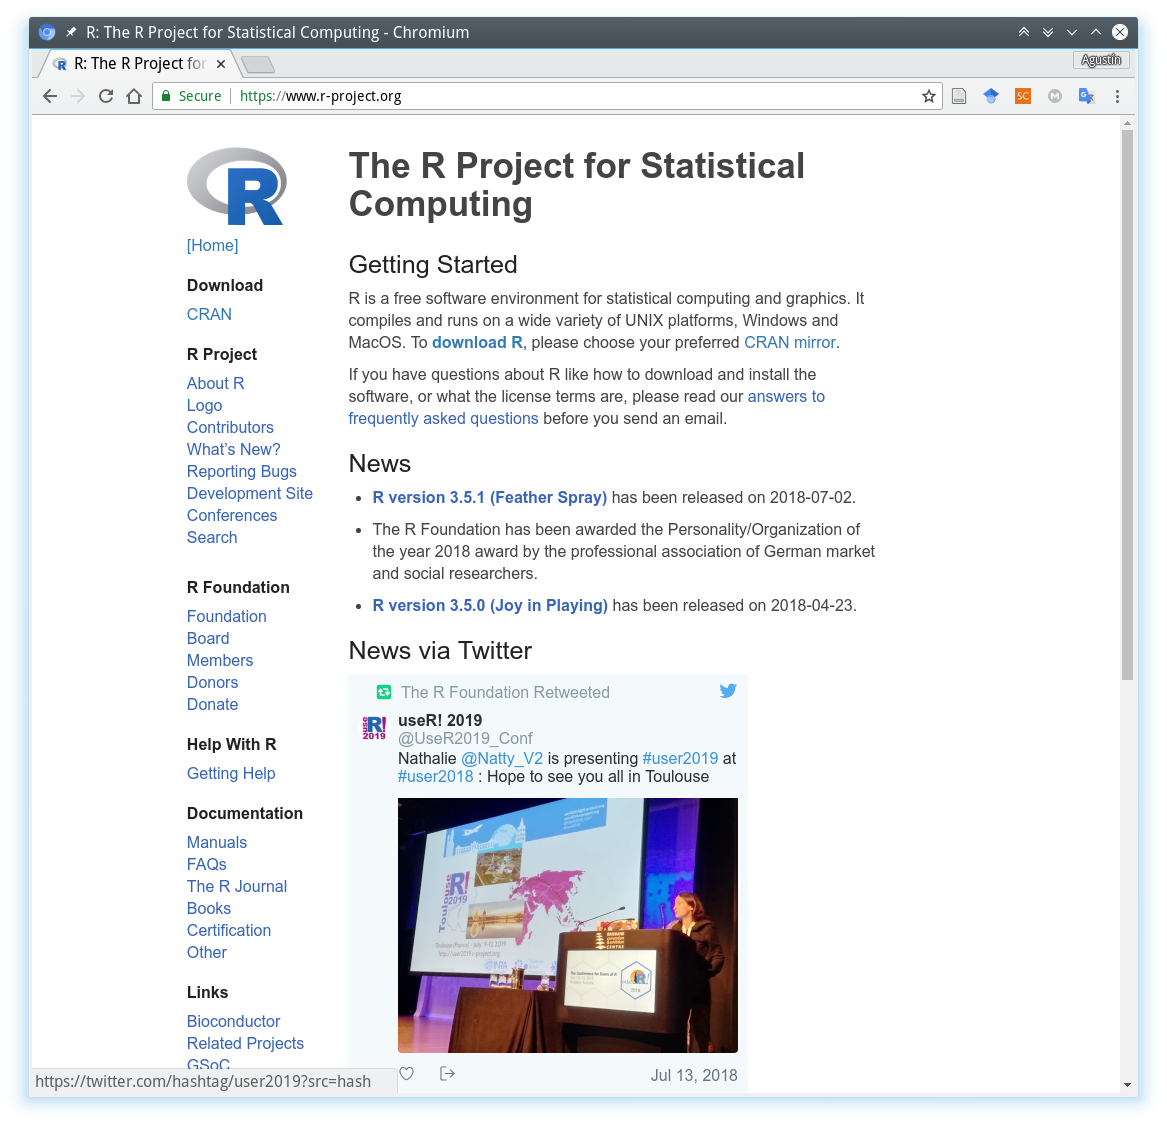
\includegraphics[width=0.75\linewidth,]{images/rproject} 

}

\caption{Página oficial de R Project}\label{fig:unnamed-chunk-16}
\end{figure}

Hoy en día, R es la \emph{lingua franca} del procesamiento y análisis
estadístico de datos, tanto en el ámbito académico como comercial dado
que es gratiuto, multiplataforma, de código abierto (\emph{open source},
liberado con licencia GNU/GPL). Esto lo convierte en un software muy
potente y que expresa el estado del arte de los métodos estadísticos ya
que la comunidad de usuarios contribuya constantemente con
funcionalidades e implementaciones de nuevos métodos y técnicas
estadísticas.

Al igual que su antecesor S, la flexibilidad y potencia de R se basa en
su interfaz de comandos (CLI, del inglés \emph{command line interface} )
que permite la ejecución de comandos de manera interactiva (en consola)
o automática mediante scritps.

\begin{figure}[h]

{\centering 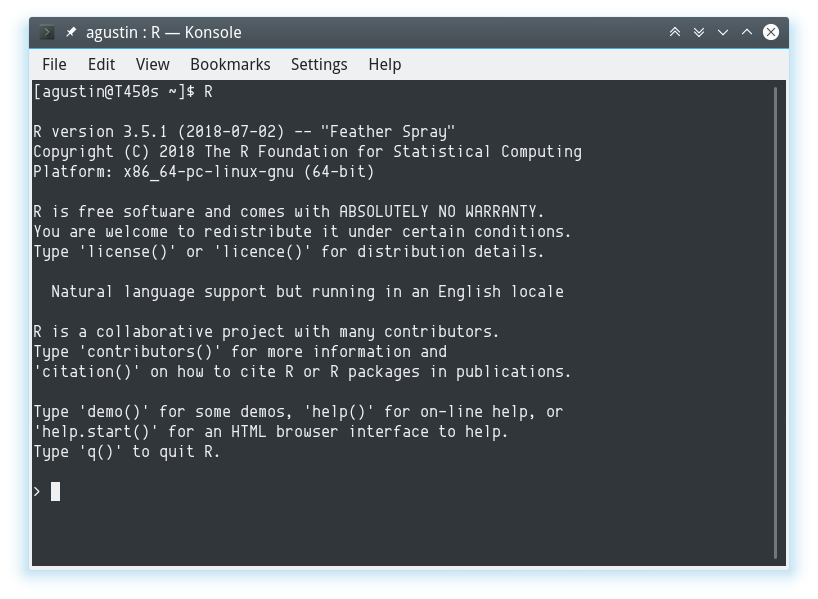
\includegraphics[width=0.75\linewidth,]{images/consola_linux} 

}

\caption{Consola o terminal de Windows, Mac OS X y Linux corriendo la última versión estable de R}\label{fig:unnamed-chunk-171}
\end{figure}
\begin{figure}[h]

{\centering 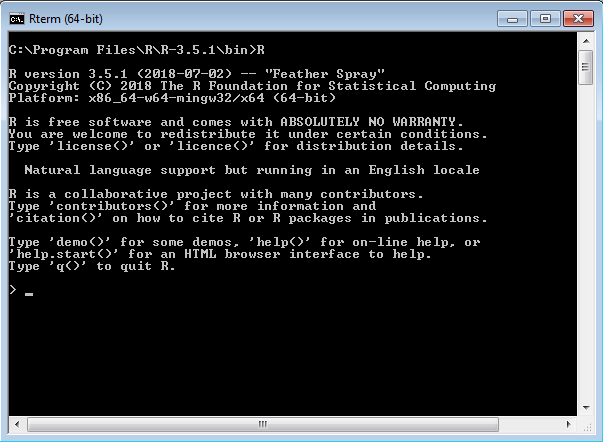
\includegraphics[width=0.75\linewidth,]{images/consola_windows} 

}

\caption{Consola o terminal de Windows, Mac OS X y Linux corriendo la última versión estable de R}\label{fig:unnamed-chunk-172}
\end{figure}

Existen algunos desarrollos de interfases gráficas (GUIs, del inglés
\emph{graphical user interface}), e.g.~RCommander, Deducer, que ofrecen
la posibilidad de, mediante menues y botones, ejecutar análisis
relativamente simples minimizando la necesidad de escribir código.

\begin{figure}[h]

{\centering 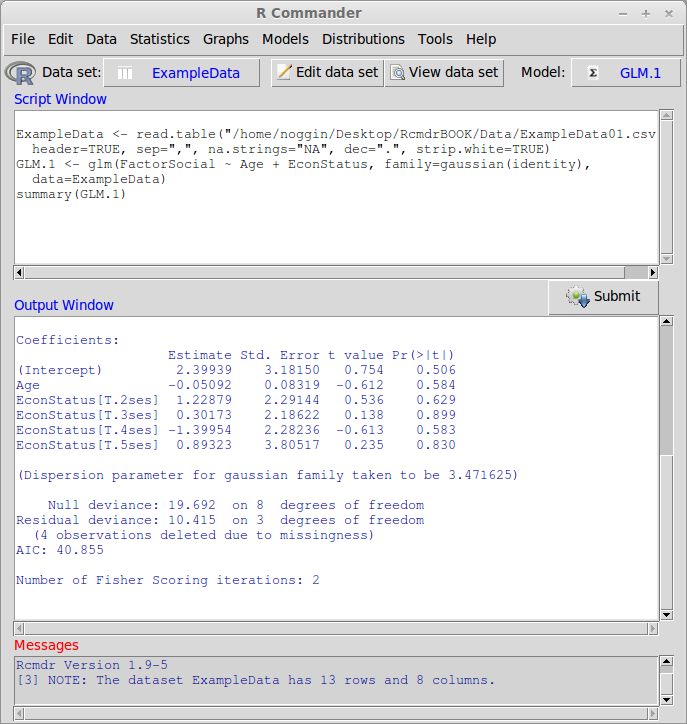
\includegraphics[width=0.75\linewidth,]{images/RcmdrBASE} 

}

\caption{Interfase de R Commander}\label{fig:unnamed-chunk-18}
\end{figure}

Por su parte, los entornos de desarrollo integrados (IDE por sus siglas
en inglés \emph{integrated development environments}) ofrecen un enfoque
intermedio con menúes o funciones asistentes que facilitan algunas
tareas generales (abrir archivos, carga de datos, exportar gráficos y
resultados) pero dejando la codificación del análisis estadístico en
manos del usuario mediante la ejecución de scripts. Entre estas
alternativas se destaca R Studio ( \url{www.rstudio.com} ) el cual
también es de código abierto (licencia GNU/GPL), multiplataforma y
ofrece una versión gratuita.

\begin{figure}[h]

{\centering \includegraphics[width=0.75\linewidth,]{images/RStudio} 

}

\caption{Interfase de R Studio}\label{fig:unnamed-chunk-19}
\end{figure}

\hypertarget{como-instalar-r-y-rstudio-1}{%
\section{¿Cómo instalar R y
RStudio?}\label{como-instalar-r-y-rstudio-1}}

RStudio requiere que el sistema tenga al menos una versión de R
instalada. Ambos softwares son multiplataforma y pueden ser ejecutados
en sistemas operativos Windows, OS X y Linux. A continuación se describe
el procedimiento para instalar R y RStudio bajo Windows.

\hypertarget{instalacion-de-r-1}{%
\subsection{Instalación de R}\label{instalacion-de-r-1}}

\begin{enumerate}
\def\labelenumi{\arabic{enumi})}
\tightlist
\item
  Descargar el archivo instalador correspondiente a la última versión
  estable de R desde el CRAN\footnote{CRAN se compone de un conjunto de
    servidores espejo distribuidos alrededor del mundo que tienen copias
    de R y sus paquetes. No es necesario escojer el espejo más cercano
    ya que el espejo nube (\url{https://cloud.r-project.org})
    automáticamente determina de que servidor conviene realizar la
    descarga.} (del inglés, \emph{Comprenhensive R Archive Network})
  visitando el siguiente
  \href{https://cloud.r-project.org/bin/windows/base/release.htm}{link}
  \footnote{Al momento de escribir estas instrucciones la última versión
    estable de R era la 3.5.1 ``Feather Spray'', por lo tanto el link
    apuntará al archivo \texttt{R-3.5.1-win.exe}.}.
\end{enumerate}

\begin{figure}[h]

{\centering 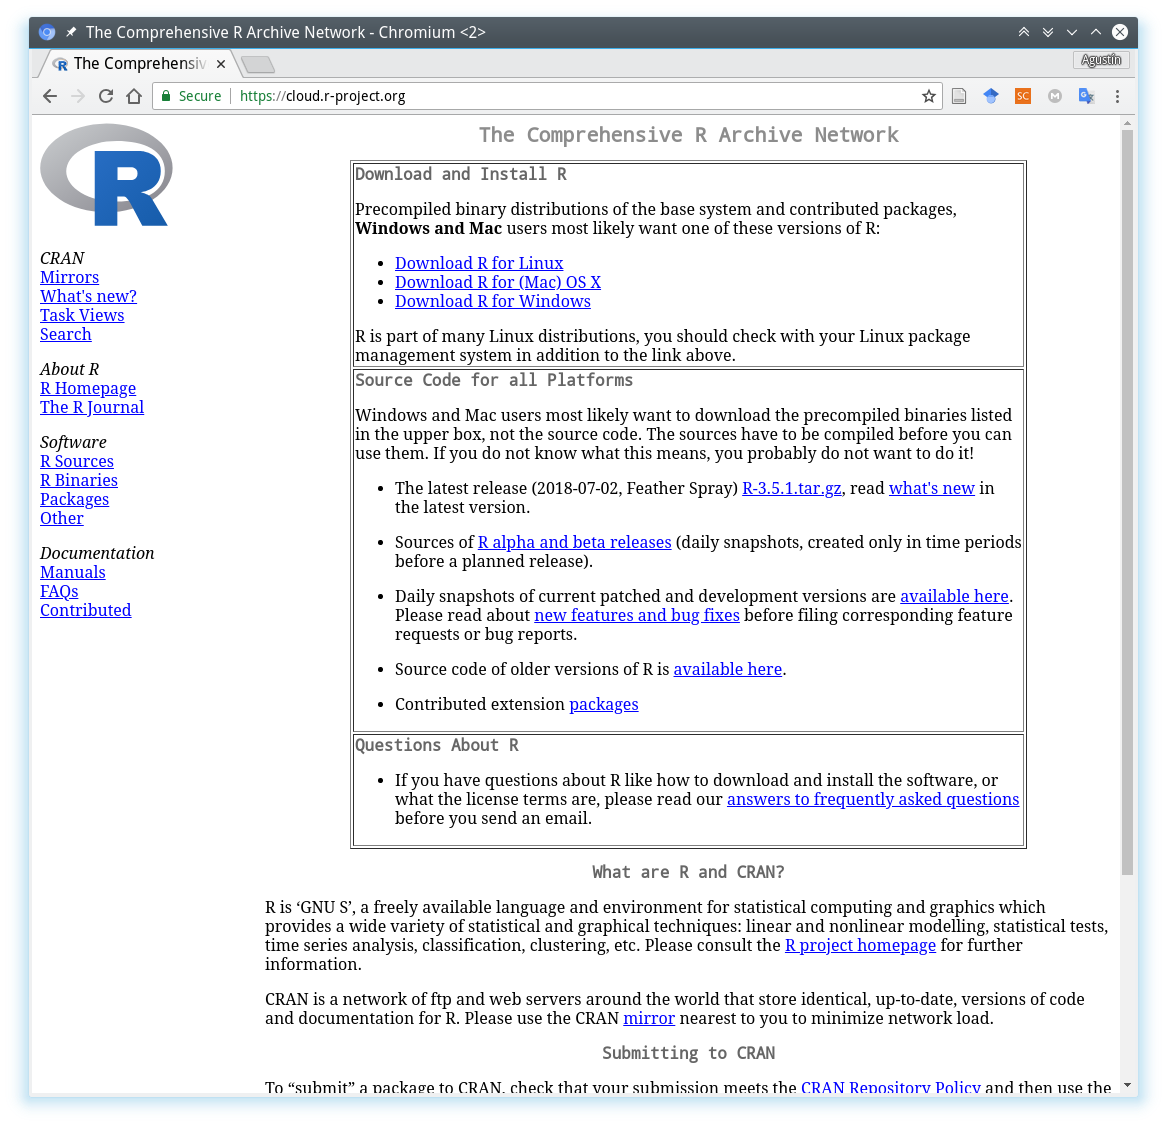
\includegraphics[width=0.75\linewidth,]{images/choose_OS} 

}

\caption{Página de descaga de R}\label{fig:unnamed-chunk-20}
\end{figure}

\begin{enumerate}
\def\labelenumi{\arabic{enumi})}
\setcounter{enumi}{1}
\item
  Una vez finalizada la descarga ejecutar el archivo \texttt{.exe} y
  seguir el asistente de instalación con todas las opciones por defecto.

  Si la instalación ha sido exitosa el el menú \emph{Inicio
  \textgreater{} Todos los Programas \textgreater{} R} se encontrarán
  dos accesos directos \texttt{R\ i386\ 3.5.1} y \texttt{R\ x64\ 3.5.1}
  los cuales permiten correre la interfase de usuario mínima que viene
  con la versión de R para Windows.
\end{enumerate}

\begin{figure}[h]

{\centering 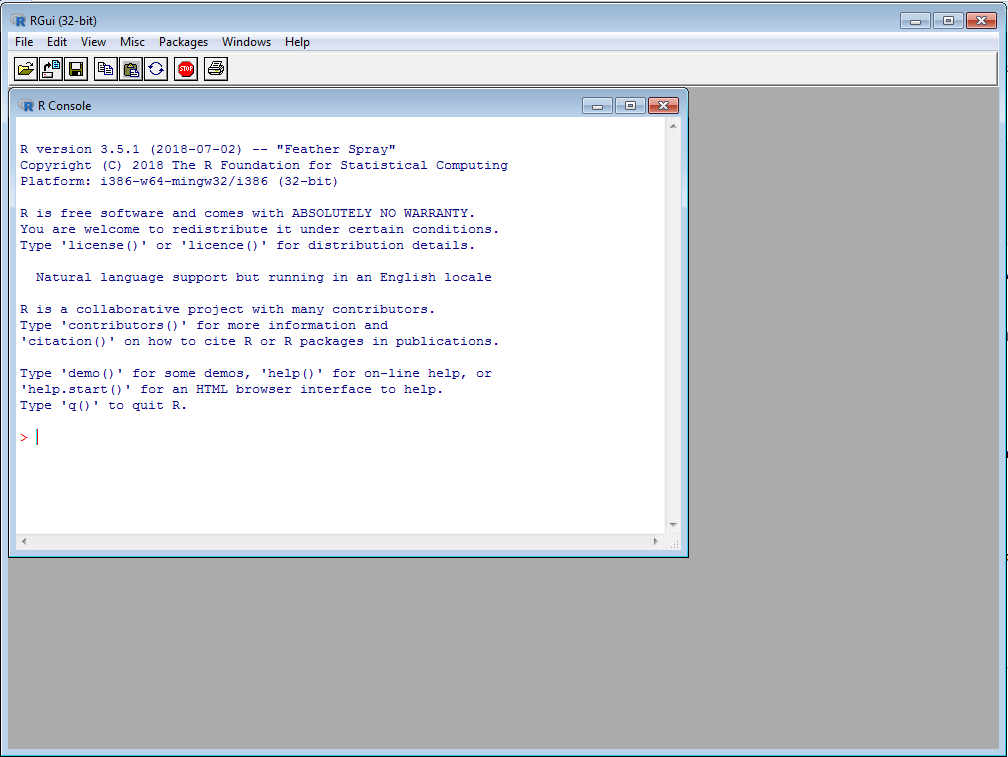
\includegraphics[width=0.75\linewidth,]{images/rgui} 

}

\caption{R GUI para Windows}\label{fig:unnamed-chunk-21}
\end{figure}

\hypertarget{instalacion-de-rstudio-1}{%
\subsection{Instalación de RStudio}\label{instalacion-de-rstudio-1}}

\begin{enumerate}
\def\labelenumi{\arabic{enumi})}
\tightlist
\item
  Ir al sitio web de descarga de RStudio:
  \url{https://www.rstudio.com/products/rstudio/download/}
\end{enumerate}

\begin{figure}[h]

{\centering 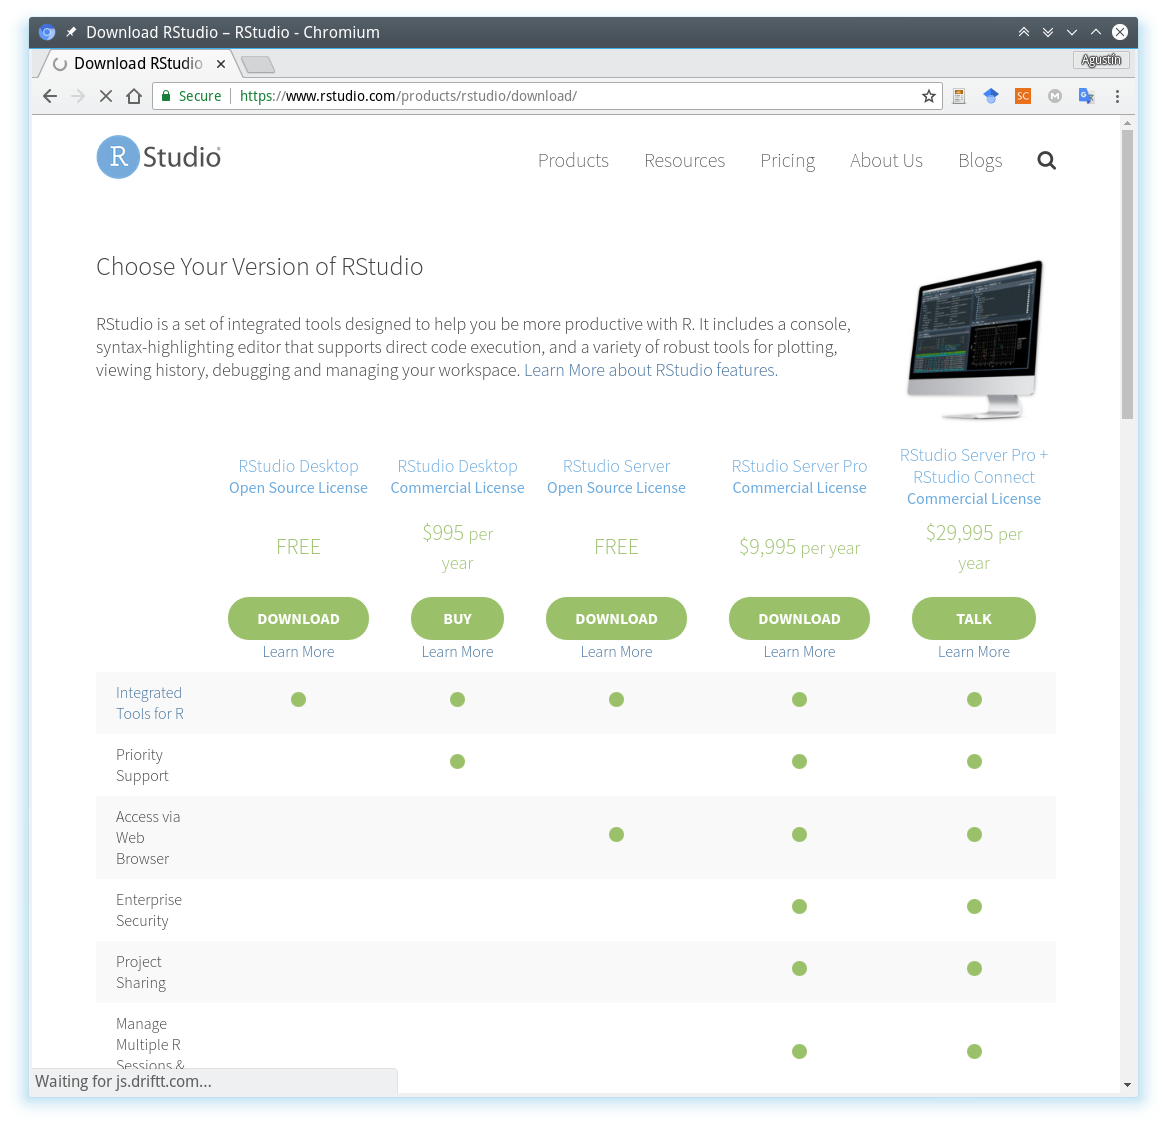
\includegraphics[width=0.75\linewidth,]{images/rstudio_download} 

}

\caption{Página principal de RStudio}\label{fig:unnamed-chunk-22}
\end{figure}

\begin{enumerate}
\def\labelenumi{\arabic{enumi})}
\setcounter{enumi}{1}
\tightlist
\item
  Descargar el archivo de instalación correspondiente a nuestra
  plataforma o sistema operativo. Por ejemplo: para Windows iniciará la
  descarga del archivo \texttt{RStudio-1.1.453.exe}
\end{enumerate}

\begin{figure}[h]

{\centering 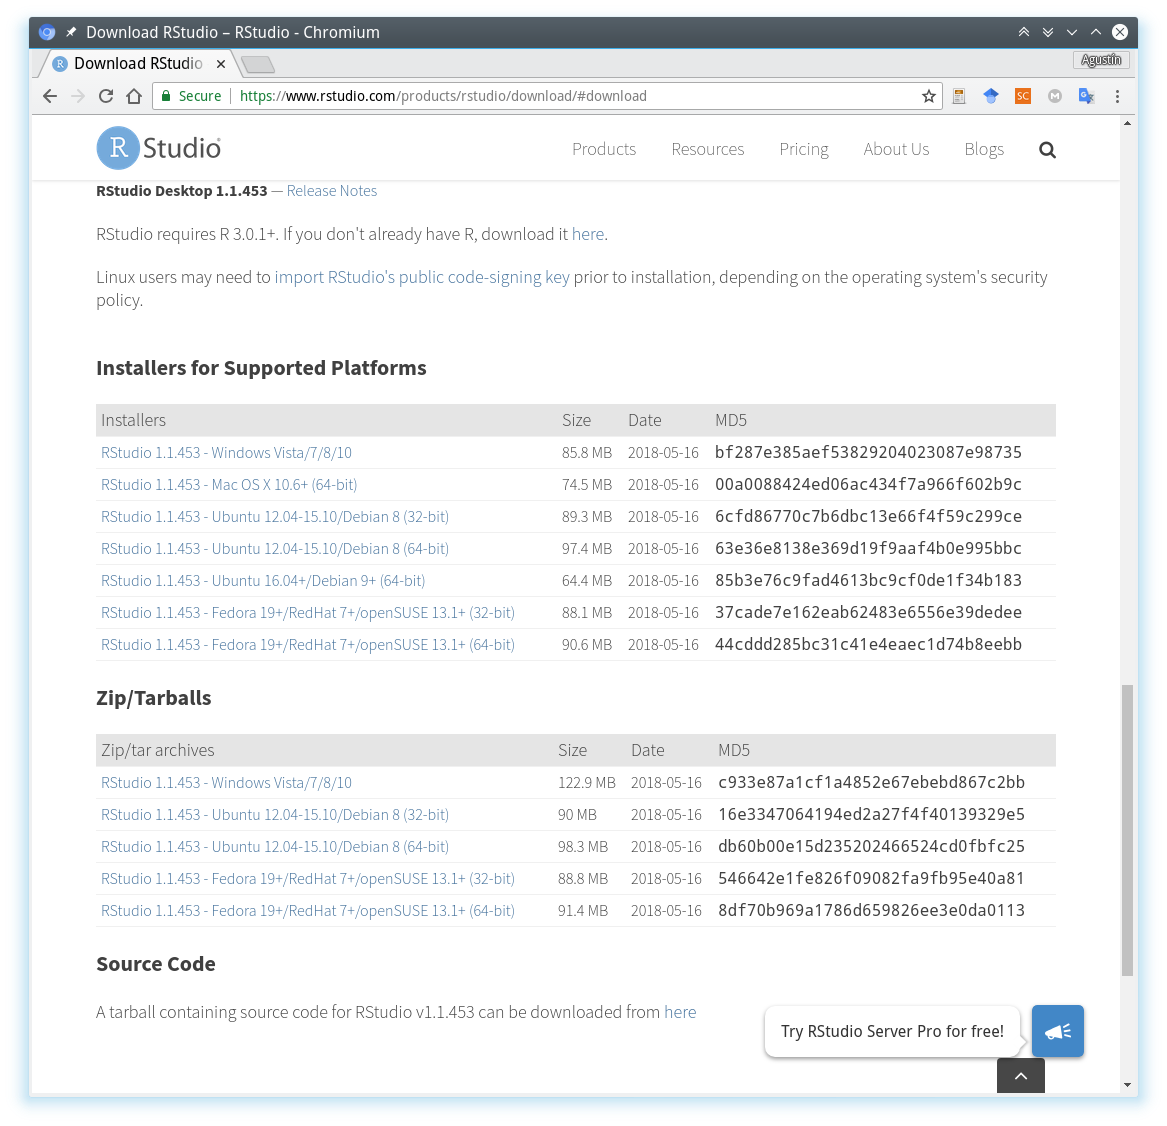
\includegraphics[width=0.75\linewidth,]{images/rstudio_download_OS} 

}

\caption{Página principal de RStudio}\label{fig:unnamed-chunk-23}
\end{figure}

\begin{enumerate}
\def\labelenumi{\arabic{enumi})}
\setcounter{enumi}{2}
\tightlist
\item
  Una vez finalizada la descarga ejecutar el archivo \texttt{.exe}
  \footnote{Al momento de escribir estas instrucciones la última versión
    estable de R Studio era la 1.1.453 por lo tanto el link apuntará al
    archivo \texttt{RStudio-1.1.453.exe}.} \texttt{RStudio-1.1.453.exe}
  y seguir el asistente de instalación con todas las opciones por
  defecto.
\end{enumerate}

Si la instalación ha sido exitosa el el menú \emph{Inicio \textgreater{}
Todos los Programas \textgreater{} R Studio} se encontrará el acceso
directo a R Studio el cual, mediante el menu contextual (botón derecho
del ratón) puede enviarse al Escritorio como acceso directo o bien
anclar al menu de Inicio o barra de acceso rápido.

Ahora sí, ya tenemos listo R y RStudio para empezar a trabajar!!

\hypertarget{revision-de-estadistica-basica}{%
\chapter{Revisión de estadística
básica}\label{revision-de-estadistica-basica}}

En este capítulo se revisarán algunos conceptos estadísticos básicos que
son fundamentales para el diseño y análisis estadísticod de experimentos

\bibliography{book.bib,packages.bib}


\end{document}
